% Options for packages loaded elsewhere
\PassOptionsToPackage{unicode}{hyperref}
\PassOptionsToPackage{hyphens}{url}
%
\documentclass[
  a4paper,
]{article}
\usepackage{amsmath,amssymb}
\usepackage{siunitx}
\newcommand{\pu}[1]{\ensuremath{\si{#1}}}
\usepackage{iftex}
\usepackage{tikz}
\ifPDFTeX
  \usepackage[T1]{fontenc}
  \usepackage[utf8]{inputenc}
  \usepackage{textcomp} % provide euro and other symbols
\else % if luatex or xetex
  \usepackage{unicode-math} % this also loads fontspec
  \defaultfontfeatures{Scale=MatchLowercase}
  \defaultfontfeatures[\rmfamily]{Ligatures=TeX,Scale=1}
\fi
\usepackage{xcoffins}
\usepackage{lmodern}

\ifPDFTeX\else
% xetex/luatex font selection
\fi
% Use upquote if available, for straight quotes in verbatim environments
\IfFileExists{upquote.sty}{\usepackage{upquote}}{}
\IfFileExists{microtype.sty}{% use microtype if available
  \usepackage[]{microtype}
  \UseMicrotypeSet[protrusion]{basicmath} % disable protrusion for tt fonts
}{}
\makeatletter
\@ifundefined{KOMAClassName}{% if non-KOMA class
  \IfFileExists{parskip.sty}{%
    \usepackage{parskip}
  }{% else
    \setlength{\parindent}{0pt}
    \setlength{\parskip}{6pt plus 2pt minus 1pt}}
}{% if KOMA class
  \KOMAoptions{parskip=half}}
\makeatother
\usepackage{xcolor}
\usepackage{minted}

% Set the `style=tango` attribute for all minted blocks.  Can still be overriden
% per block (e.g., you want to change just one).  Run `pygmentize -L` to see
% all available options.
\usemintedstyle{tango}

% Depending on which pygments style you choose, comments and preprocessor
% directives may be italic.  The `tango` style is one of these.  This disables
% all italics in the `minted` environment.
\BeforeBeginEnvironment{minted}{\selectlanguage{english}}
\AtBeginEnvironment{minted}{\let\itshape\relax}
\AfterEndEnvironment{minted}{\selectlanguage{hebrew}}

% This disables italics for the `\mintinline` commands.
% Credit: https://tex.stackexchange.com/a/469702/113687
\usepackage{xpatch}
\xpatchcmd{\mintinline}{\begingroup}{\begingroup\let\itshape\relax}{}{}


\usepackage{graphicx}
\makeatletter
\def\maxwidth{\ifdim\Gin@nat@width>\linewidth\linewidth\else\Gin@nat@width\fi}
\def\maxheight{\ifdim\Gin@nat@height>\textheight\textheight\else\Gin@nat@height\fi}
\makeatother
% Scale images if necessary, so that they will not overflow the page
% margins by default, and it is still possible to overwrite the defaults
% using explicit options in \includegraphics[width, height, ...]{}
\setkeys{Gin}{width=\maxwidth,height=\maxheight,keepaspectratio}
% Set default figure placement to htbp
\makeatletter
\def\fps@figure{H}
\makeatother
\usepackage{color}
\usepackage{transparent}
\usepackage[inkscapelatex=false, inkscapeformat=png]{svg}
\setlength{\emergencystretch}{3em} % prevent overfull lines
\providecommand{\tightlist}{%
  \setlength{\itemsep}{0pt}\setlength{\parskip}{0pt}}
\setcounter{secnumdepth}{-\maxdimen} % remove section numbering
\ifLuaTeX
  \usepackage{selnolig}  % disable illegal ligatures
\fi
\ifPDFTeX
  \TeXXeTstate=1
  \newcommand{\RL}[1]{\beginR #1\endR}
  \newcommand{\LR}[1]{\beginL #1\endL}
  \newenvironment{RTL}{\beginR}{\endR}
  \newenvironment{LTR}{\beginL}{\endL}
\fi
\usepackage{bookmark}
\IfFileExists{xurl.sty}{\usepackage{xurl}}{} % add URL line breaks if available
\urlstyle{same}
\hypersetup{
  pdflang={he},
  hidelinks,
  pdfcreator={LaTeX via pandoc}}

\usepackage{fvextra}
\usepackage{polyglossia}
\setdefaultlanguage{hebrew}
\setotherlanguage{english}
\usepackage{fontspec}
\setmainfont{David CLM} % main font
\setsansfont{David CLM} % sans serif font
\newfontfamily\hebrewfonttt[Script=Hebrew]{David CLM} % monospace font

\author{}
\date{}

\begin{document}

\NewCoffin\Output   %Coffin to hold the others 
\NewCoffin\Callout % Callout definition ...
\NewCoffin\BackFrame % Background: green rectangle
\NewCoffin\SideRule  %lateral left border


\newcommand{\SetCallout}[2]{%
    \SetHorizontalCoffin\Output{} % It will be the reference point join the others  
    \SetVerticalCoffin\Callout{\linewidth-20pt}{\textbf{#1} \\ #2 \leavevmode \\ \\}

    %% Make both \BackFrame & SideRule heights = height of Callout + 1*baselineskip
    \SetHorizontalCoffin\BackFrame{
      \begingroup
      \color{green!30!gray!15}\rule{\linewidth}{\CoffinTotalHeight\Callout}
      \endgroup
    }    
    \SetHorizontalCoffin\SideRule{
      \begingroup  
      \color{green!50!black}\rule{3pt}{\CoffinTotalHeight\Callout}
      \endgroup
    } %vertical side rule 

    %% Assembly Coffins
    \JoinCoffins*\Output[l,t]\Callout[l,t](10pt,-\baselineskip) %attach left-top corner of Callout to idem of Output
    \JoinCoffins*\Output[l,t]\SideRule[l,t] %attach left-top corner of  SideRule to idem of Output
    \JoinCoffins*\Output[l,t]\BackFrame[l,t] %attach left-top corner of BackFrame  to idem of Output
    %% Typeset ooutput
    \noindent\TypesetCoffin\Output % at the text insertion point. It is not a float.
    \vspace*{\CoffinTotalHeight\Callout}\bigskip %make some room for Output
}

\section{כותרת 1}\label{ux5dbux5d5ux5eaux5e8ux5ea-1}

לורם איפסום דולור סיט אמט, קונסקטורר אדיפיסינג אלית נולום ארווס סאפיאן -
פוסיליס קוויס, אקווזמן לורם איפסום דולור סיט אמט, קונדימנטום קורוס
בליקרה, נונסטי קלובר בריקנה סטום, לפריקך תצטריק לרטי.

לורם איפסום דולור סיט אמט, קונסקטורר אדיפיסינג אלית נולום ארווס סאפיאן -
פוסיליס קוויס, אקווזמן לורם איפסום דולור סיט אמט, קונדימנטום קורוס
בליקרה, נונסטי קלובר בריקנה סטום, לפריקך תצטריק לרטי. לורם איפסום דולור
סיט אמט, קונסקטורר אדיפיסינג אלית נולום ארווס סאפיאן - פוסיליס קוויס,
אקווזמן לורם איפסום דולור סיט אמט, קונדימנטום קורוס בליקרה, נונסטי קלובר
בריקנה סטום, לפריקך תצטריק לרטי.

\subsection{תת כותרת 2}\label{ux5eaux5ea-ux5dbux5d5ux5eaux5e8ux5ea-2}

רשימה ממוספרת:

\begin{enumerate}
\def\labelenumi{\arabic{enumi}.}
\tightlist
\item
  לורם איפסום דולור סיט אמט, קונסקטורר אדיפיסינג אלית נולום ארווס סאפיאן
  - פוסיליס קוויס,
\item
  אקווזמן לורם איפסום דולור סיט אמט, קונדימנטום קורוס בליקרה, נונסטי
  קלובר בריקנה סטום,
\item
  לפריקך תצטריק לרטי.
\end{enumerate}

רשימת נקודות: - לורם איפסום דולור סיט אמט, קונסקטורר אדיפיסינג אלית
נולום ארווס סאפיאן - פוסיליס קוויס, - אקווזמן לורם איפסום דולור סיט אמט,
קונדימנטום קורוס בליקרה, נונסטי קלובר בריקנה סטום, - לפריקך תצטריק לרטי.

\section{בלוק קוד}\label{ux5d1ux5dcux5d5ux5e7-ux5e7ux5d5ux5d3}

פייתון:

\begin{minted}[breaklines,autogobble]{python}
import numpy as np
import sympy as sp
import matplotlib.pyplot as plt

def composite_trapezoidal(f, a, b, n):
    h = (b - a) / n
    s = f(a) + f(b)
    for i in range(1, n):
        s += 2 * f(a + i * h)
    return s * h / 2

def composite_simpsons(f, a, b, n):
    h = (b - a) / n
    s = f(a) + f(b)
    for i in range(1, n):
        if i % 2 == 0:
            s += 2 * f(a + i * h)
        else:
            s += 4 * f(a + i * h)
    return s * h / 3

def richardson_extrapolation_simp(f, a, b, n):
    I1 = composite_simpsons(f, a, b, n)
    I2 = composite_simpsons(f, a, b, 2*n)
    return (16*I2 - I1) / 15

f = lambda x: (x+1)/(4*x+3)
a = 0
b = 6
\end{minted}

מה לגבי \mintinline[]{text}{code} בתוך שורה?

\section{מתמטיקה}\label{ux5deux5eaux5deux5d8ux5d9ux5e7ux5d4}

סתם \mintinline[]{text}{gathered}:

\[\begin{gathered}
0=-w+{h}_{1}-{h}_{2} \\
w={h}_{1}-{h}_{2}
\end{gathered}\]

סתם טבלה (\mintinline[]{text}{array}): \[\begin{array}{c|c|c|c|c}
\text{state} & p[\pu{kPa}] & T[^{\circ}\pu{C}] &  h[\pu{kJ/kg}]  & s[\pu{kJ/kg*K}] \\
\hline 1  & 800 & 500  & 3480.6 & 7.8673 \\ 
\hline 2 & 200 & 309.74 &  3091.75  & 7.9245
\end{array}\]

\section{קולאאוס
(Callout)}\label{ux5e7ux5d5ux5dcux5d0ux5d0ux5d5ux5e1-callout}

\SetCallout{הערה:}{ לורם איפסום דולור סיט אמט, קונסקטורר אדיפיסינג אלית
נולום ארווס סאפיאן - פוסיליס קוויס, אקווזמן לורם איפסום דולור סיט אמט,
קונדימנטום קורוס בליקרה, נונסטי קלובר בריקנה סטום, לפריקך תצטריק לרטי.}

כחלק מפסקה:

\SetCallout{הערה:}{לורם איפסום דולור סיט אמט, קונסקטורר אדיפיסינג אלית
נולום ארווס סאפיאן - פוסיליס קוויס, אקווזמן לורם איפסום דולור סיט אמט,
קונדימנטום קורוס בליקרה, נונסטי קלובר בריקנה סטום, לפריקך תצטריק לרטי.}

כחלק ממספור:

\begin{enumerate}
\def\labelenumi{\arabic{enumi}.}
\tightlist
\item
  בלה בלה בלה

  \SetCallout{הערה:}{לורם איפסום דולור סיט אמט, קונסקטורר אדיפיסינג אלית
  נולום ארווס סאפיאן - פוסיליס קוויס, אקווזמן לורם איפסום דולור סיט אמט,
  קונדימנטום קורוס בליקרה, נונסטי קלובר בריקנה סטום, לפריקך תצטריק
  לרטי.}
\end{enumerate}

קולאאוס מסוג אחר:

\SetCallout{משפט:}{ לורם איפסום דולור סיט אמט, קונסקטורר אדיפיסינג אלית
נולום ארווס סאפיאן - פוסיליס קוויס, אקווזמן לורם איפסום דולור סיט אמט,
קונדימנטום קורוס בליקרה, נונסטי קלובר בריקנה סטום, לפריקך תצטריק לרטי.}

\section{תמונה}\label{ux5eaux5deux5d5ux5e0ux5d4}

תמונה:

\begin{figure}
\centering
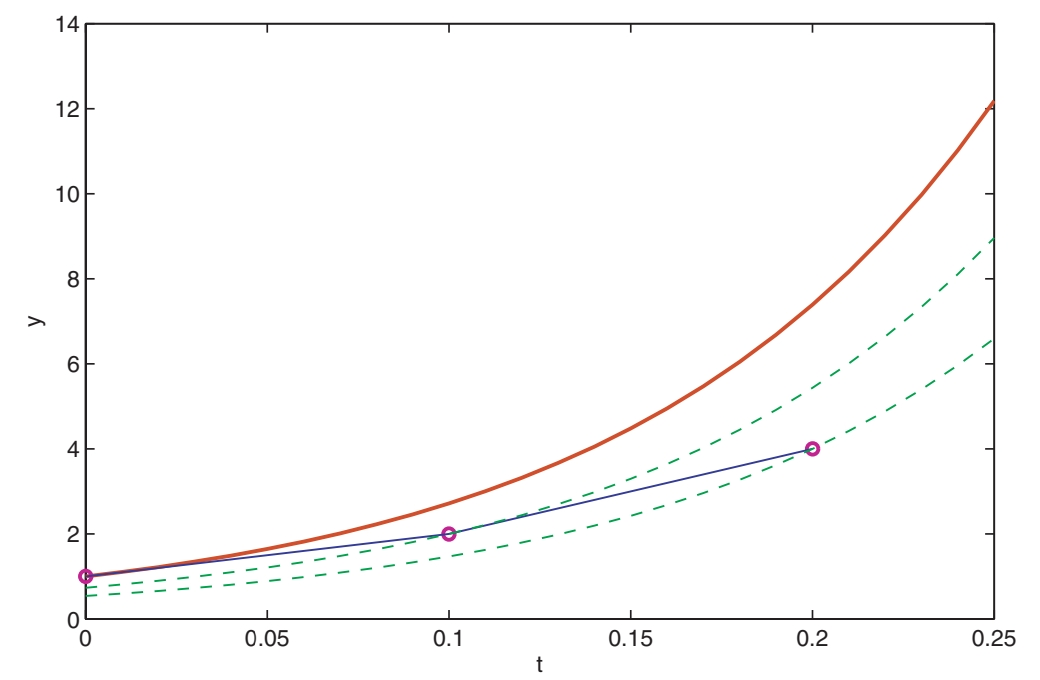
\includegraphics[width=0.75\textwidth,height=0.4\textheight]{NUM1/NUM1_011/Screenshot_20240322_182502_OneDrive.jpg}
\caption{}
\end{figure}

תמונה כחלק מפסקה (\mintinline[]{text}{inline}):

\begin{figure}
\centering
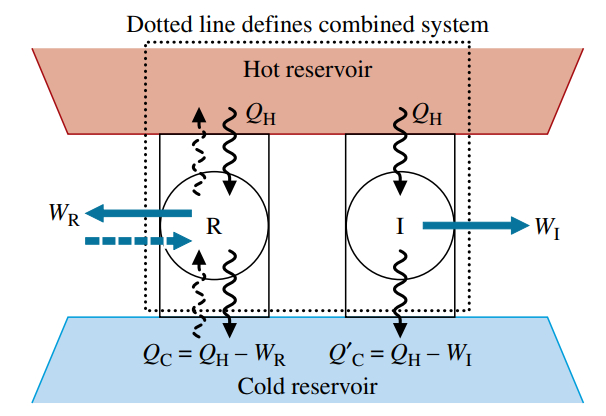
\includegraphics[width=0.75\textwidth,height=0.4\textheight]{THE1/THE1_005/Pasted image 20240223092520.png}
\caption{}
\end{figure}

תמונה עם caption:

\begin{figure}
\centering
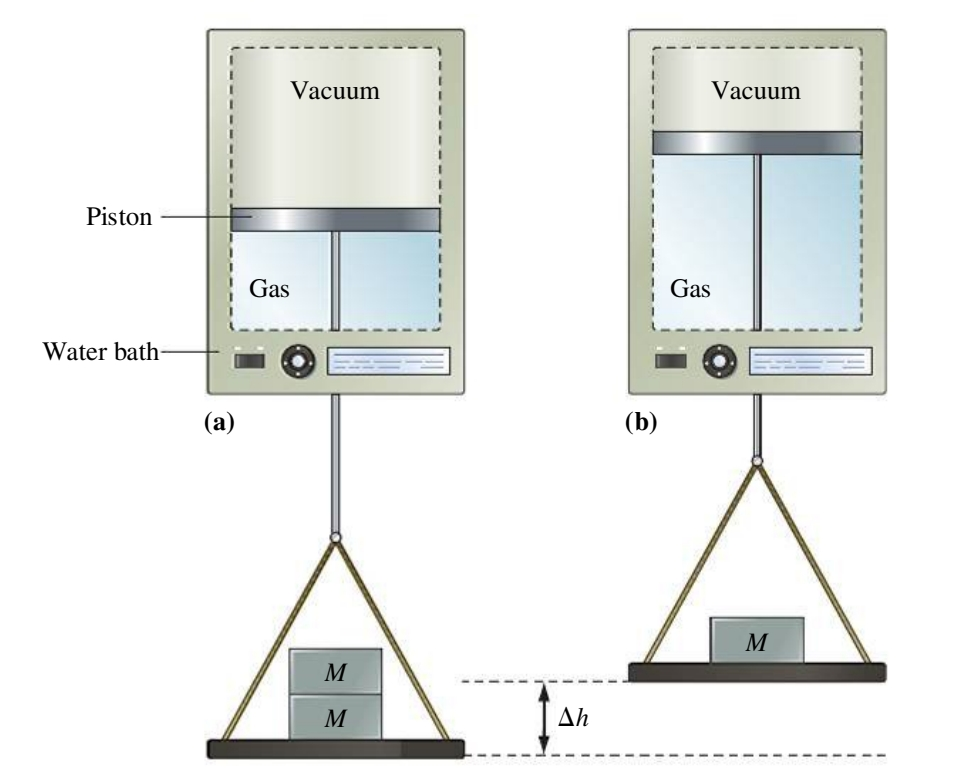
\includegraphics[width=0.75\textwidth,height=0.4\textheight]{GCH1/GCH1_004/Screenshot_20230127_102808_Microsoft 365 (Office).jpg}
\caption{וואו זה מאוד מעניין.}
\end{figure}

תמונת \mintinline[]{text}{svg}:

\begin{figure}
\centering
\includesvg[width=0.75\textwidth,height=0.4\textheight]{THE1/THE1_HW008/THE1_HW008 תרגיל בית 8 2024-03-24 00.41.23.excalidraw.svg}
\caption{THE1/THE1\_HW008/THE1\_HW008 תרגיל בית 8 2024-03-24
00.41.23.excalidraw.svg}
\end{figure}

תמונת \mintinline[]{text}{svg} עם caption:

\begin{figure}
\centering
\includesvg[width=0.75\textwidth,height=0.4\textheight]{THE1/THE1_HW008/THE1_HW008 תרגיל בית 8 2024-03-24 14.23.59.excalidraw.svg}
\caption{וואו זה מאוד מעניין.}
\end{figure}

תמונה בתוך קולאאוט:

\SetCallout{הערה:}{
  \begin{figure}
  \centering
  \begin{tikzpicture}[blend mode=multiply]
  \node{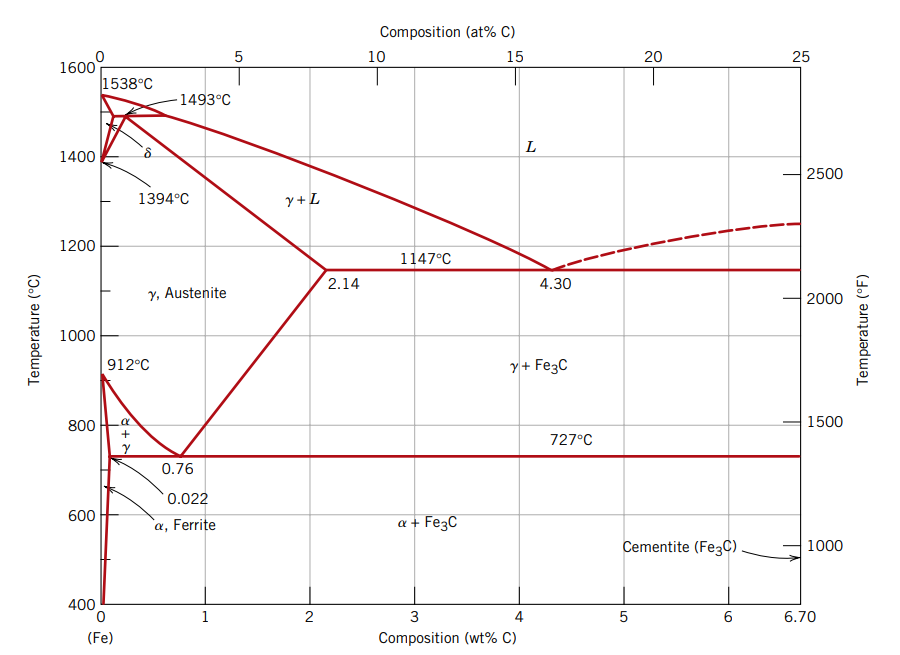
\includegraphics[width=0.75\textwidth,height=0.4\textheight]{IMT1/IMT1_005/Pasted image 20230514202911.png}};
  \end{tikzpicture}
\end{figure}}

תמונה בתוך קולאאוט עם caption:

\SetCallout{הערה:}{וואו קבלו קטע:
\textgreater{}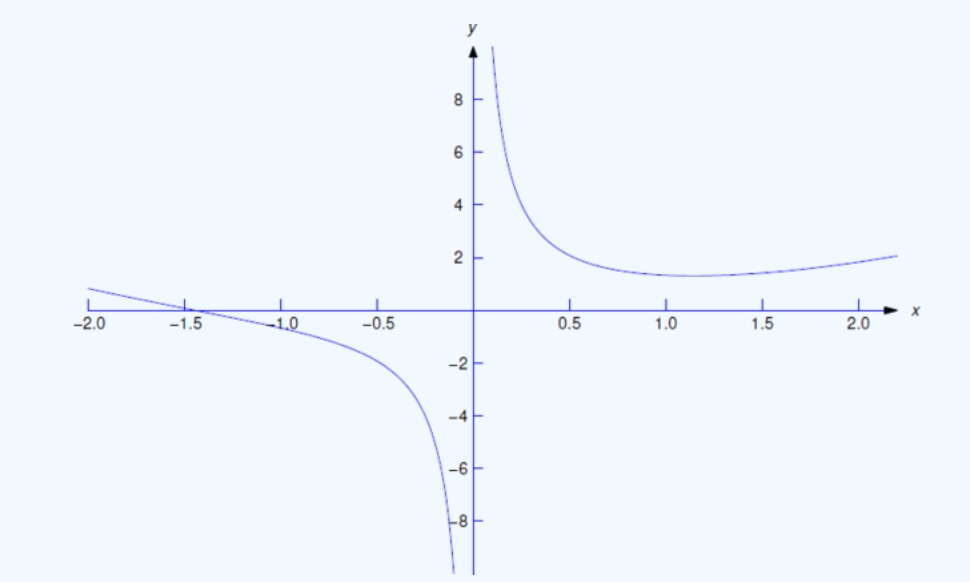
\includegraphics[width=0.75\textwidth,height=0.4\textheight]{DEQ1/DEQ1_001/Screenshot_20230426_235017_Chrome.jpg}
\textgreater\textgreater וואו איזה מעניין}

\end{document}
